\documentclass{beamer}

%Russian-specific packages
%--------------------------------------
\usepackage[T2A]{fontenc}
\usepackage[utf8]{inputenc}
\usepackage[english,main=russian]{babel}
%--------------------------------------

\usepackage{graphicx}
\usepackage{amssymb,amsmath}
\usepackage{pgfplots, pgfplotstable}
\pgfplotsset{compat=newest}

\graphicspath{{logo/}{pics/}}
\beamertemplatenavigationsymbolsempty{}
\setbeamertemplate{footline}[frame number]
\setbeamerfont{footline}{size={\fontsize{10}{12}}}

\usepackage{pgfplots, pgfplotstable}
\usepgfplotslibrary{fillbetween}
\pgfplotsset{compat=newest}

\makeatletter
\pgfplotsset{%
    /pgfplots/flexible xticklabels from table/.code n args={3}{%
        \pgfplotstableread[#3]{#1}\coordinate@table
        \pgfplotstablegetcolumn{#2}\of{\coordinate@table}\to\pgfplots@xticklabels
        \let\pgfplots@xticklabel=\pgfplots@user@ticklabel@list@x
    }
}
\makeatother%
\definecolor{basicno}{rgb}{0.624,0.0,0.0}
\definecolor{basicsome}{rgb}{0.424,0.0,0.0}
\definecolor{random}{rgb}{0.0,0.100,0.424}
\definecolor{gena}{rgb}{0.0,0.100,0.624}
\definecolor{heuno}{rgb}{0.2,0.524,0.2}
\definecolor{heusome}{rgb}{0.2,0.424,0.2}
\definecolor{heumore}{rgb}{0.1,0.324,0.1}

\newcommand{\addplottime} [2] {%
\addplot 
    [color=#2, fill=#2, fill opacity=0.33]
    plot [error bars/.cd, error bar style={line width=1pt}, y dir = both, y explicit]
    table[x expr=\coordindex, y=mean_time, y error=std_time]{#1};
}

\newenvironment{timeaxis} [3] {%
\begin{axis}[
    enlarge x limits=0.2,
    ybar=0pt, 
    width=#1,
    height=#2,
    bar width=8pt,
    ymin=0,
    xlabel=Датасет,
    ylabel=Время работы в сек,
    flexible xticklabels from table={#3}{algo}{col sep=comma},
    xticklabel style={text height=1.5ex, font=\tiny}, % To make sure the text labels are nicely aligned
    xtick=data,
    legend cell align={left},
    % legend style={at={(0.02,0.98)},anchor=north west},
]
}{%
\end{axis}
}

\newcommand{\timebig} [2] {%
\pgfplotstableread[col sep=comma]{../data/big/basic-00.csv}\basicno
\pgfplotstableread[col sep=comma]{../data/big/basic-05.csv}\basicsome
\pgfplotstableread[col sep=comma]{../data/big/heuristic-00.csv}\heuno
\pgfplotstableread[col sep=comma]{../data/big/heuristic-05.csv}\heusome
\pgfplotstableread[col sep=comma]{../data/big/heuristic-15.csv}\heumore
\pgfplotstableread[col sep=comma]{../data/big/random.csv}\random

\begin{tikzpicture}
\begin{timeaxis}{#1}{#2}{../data/big/heuristic-15.csv}

\addplottime{\basicno}{basicno}
\addplottime{\basicsome}{basicsome}
\addplottime{\random}{random}
\addplottime{\heuno}{heuno}
\addplottime{\heusome}{heusome}
\addplottime{\heumore}{heumore}

\legend{%
    Ветви/границы, 
    Ветви/границы с $<5\%$, 
    Случайный, 
    Ветви/границы + эвристика, 
    Ветви/границы + эвристика с $<5\%$, 
    Ветви/границы + эвристика с $<15\%$ 
}

\end{timeaxis}
\end{tikzpicture}
}

\newcommand{\timeeasy} [2] {%
\pgfplotstableread[col sep=comma]{../data/easy/basic-00.csv}\basicno
\pgfplotstableread[col sep=comma]{../data/easy/basic-05.csv}\basicsome
\pgfplotstableread[col sep=comma]{../data/easy/heuristic-00.csv}\heuno
\pgfplotstableread[col sep=comma]{../data/easy/heuristic-05.csv}\heusome
\pgfplotstableread[col sep=comma]{../data/easy/heuristic-15.csv}\heumore
\pgfplotstableread[col sep=comma]{../data/easy/random.csv}\random

\begin{tikzpicture}
\begin{timeaxis}{#1}{#2}{../data/easy/heuristic-15.csv}

\addplottime{\basicno}{basicno}
\addplottime{\basicsome}{basicsome}
\addplottime{\random}{random}
\addplottime{\heuno}{heuno}
\addplottime{\heusome}{heusome}
\addplottime{\heumore}{heumore}

\legend{%
    Ветви/границы, 
    Ветви/границы с $<5\%$, 
    Случайный, 
    Ветви/границы + эвристика, 
    Ветви/границы + эвристика с $<5\%$, 
    Ветви/границы + эвристика с $<15\%$ 
}

\end{timeaxis}
\end{tikzpicture}
}

\newcommand{\timetrees} [2] {%
\pgfplotstableread[col sep=comma]{../data/trees/basic-00.csv}\basicno
\pgfplotstableread[col sep=comma]{../data/trees/basic-05.csv}\basicsome
\pgfplotstableread[col sep=comma]{../data/trees/heuristic-00.csv}\heuno
\pgfplotstableread[col sep=comma]{../data/trees/heuristic-05.csv}\heusome
\pgfplotstableread[col sep=comma]{../data/trees/heuristic-15.csv}\heumore
\pgfplotstableread[col sep=comma]{../data/trees/random.csv}\random

\begin{tikzpicture}
\begin{timeaxis}{#1}{#2}{../data/trees/heuristic-15.csv}

% \addplottime{\basicno}{basicno}
% \addplottime{\basicsome}{basicsome}
\addplottime{\random}{random}
\addplottime{\heuno}{heuno}
\addplottime{\heusome}{heusome}
\addplottime{\heumore}{heumore}

\legend{%
    % Ветви/границы, 
    % Ветви/границы с $<5\%$, 
    Случайный, 
    Ветви/границы + эвристика, 
    Ветви/границы + эвристика с $<5\%$, 
    Ветви/границы + эвристика с $<15\%$ 
}

\end{timeaxis}
\end{tikzpicture}
}

\newcommand{\addploterror}[2] {% 
\addplot 
    [color=#2, fill=#2, fill opacity=0.33]
    plot [error bars/.cd, error bar style={line width=1pt}, y dir = both, y explicit] 
    table[x expr=\coordindex, y=mean_error, y error=std_error]{#1}; 
}

\newenvironment{erroraxis}[2] {% 
\begin{axis}[
    ytick={0,0.1,...,0.9},
    enlarge x limits=0.2,
    ybar=0pt, 
    width=#1,
    height=#2,
    bar width=8pt,
    ymin=0,
    xlabel=Датасет,
    ylabel=Отоносительная погрешность,
    flexible xticklabels from table={../data/easy/heuristic-15.csv}{algo}{col sep=comma},
    xticklabel style={text height=1.5ex, font=\tiny}, % To make sure the text labels are nicely aligned
    xtick=data,
    legend style={at={(0.02,0.98)},anchor=north west},
]
}{%
\end{axis}
}

\newcommand{\errorbig}[2] {%
\pgfplotstableread[col sep=comma]{../data/extra/heuristic-05.csv}\heusome
\pgfplotstableread[col sep=comma]{../data/extra/heuristic-15.csv}\heumore
\pgfplotstableread[col sep=comma]{../data/extra/random.csv}\random

\begin{tikzpicture}
\begin{erroraxis}{#1}{#2}

\addploterror{\random}{random} 
\addploterror{\heusome}{heusome}
\addploterror{\heumore}{heumore}

\legend{%
    Случайный, 
    Эвристика с $<5\%$, 
    Эвристика с $<15\%$ 
}

\end{erroraxis}
\end{tikzpicture} 
}

\newcommand{\erroreasy}[2] {%
\pgfplotstableread[col sep=comma]{../data/easy/basic-05.csv}\basicsome
\pgfplotstableread[col sep=comma]{../data/easy/heuristic-05.csv}\heusome
\pgfplotstableread[col sep=comma]{../data/easy/heuristic-15.csv}\heumore
\pgfplotstableread[col sep=comma]{../data/easy/random.csv}\random

\begin{tikzpicture} 
\begin{erroraxis}{#1}{#2}

\addploterror{\basicsome}{basicsome}
\addploterror{\random}{random}
\addploterror{\heusome}{heusome}
\addploterror{\heusome}{heumore}

\legend{%
    Перебор с $<5\%$, 
    Случайный, 
    Эвристика с $<5\%$, 
    Эвристика с $<15\%$ 
}

\end{erroraxis}
\end{tikzpicture}
}

\newcommand{\errortimeaddplot}[2] {%
\addplot 
    [scatter, color=#2, style={ultra thick}] 
    table[x=algo, y=mean_time]{#1};
\addplot 
    [name path=upper, color=#2] 
    table[x=algo, y expr=\thisrow{mean_time}-\thisrow{std_time}]{#1};
\addplot 
    [name path=lower, color=#2] 
    table[x=algo, y expr=\thisrow{mean_time}+\thisrow{std_time}]{#1};
\addplot 
    [fill, fill opacity=0.2, color=#2] 
    fill between[of=upper and lower];
}

\newcommand{\errortotime}[2] {%
\pgfplotstableread[col sep=comma]{../data/datasets/time_to_error/diabetes70-None.csv}\diabet
\pgfplotstableread[col sep=comma]{../data/datasets/time_to_error/kin8nm30-None.csv}\kinmerrtime
% \pgfplotstableread[col sep=comma]{../data/datasets/time_to_error/house_8L37-None.csv}\house

\begin{tikzpicture}
\begin{axis}[
    xtick={0.00,0.05,0.10,0.15,0.20,0.25},
    x tick label style={/pgf/number format/.cd,
            fixed, fixed zerofill, precision=2, /tikz/.cd},
    enlarge x limits=0.2,
    width=#1,
    height=#2,
    ymin=0,
    xlabel=Заданная допутсимая погрешность алгоритма,
    ylabel=Время работы в сек.,
    scatter/classes={a={mark=o}},
]

\errortimeaddplot{\diabet}{heusome}
\errortimeaddplot{\kinmerrtime}{basicno}
% \errortimeaddplot{\house}{random}

\legend{%
    diabetes-70 деревьев,,,,
    kin8nm-30 деревьев,,,,
    house\_8L-37 деревьев,
}

\end{axis}
\end{tikzpicture}
}

\newcommand{\addplotsmac}[5] {%
\addplot 
    [scatter, color=#2]
    plot [error bars/.cd, error bar style={line width=1pt}, y dir = both,
    y explicit] table[x index=#3, y expr=1-\thisrow{#4}, y error index=#5]{#1}; 
}

\newcommand{\smacsize} [2] {%
\pgfplotstableread[col sep=comma, header=false]{../data/smac/limits/new_iris_forest.csv}\forestiris
\pgfplotstableread[col sep=comma, header=false]{../data/smac/limits/new_iris_random.csv}\randomiris
\pgfplotstableread[col sep=comma, header=false]{../data/smac/limits/new_leter_forest.csv}\forestletter
\pgfplotstableread[col sep=comma, header=false]{../data/smac/limits/new_leter_random.csv}\randomletter
\pgfplotstableread[col sep=comma, header=false]{../data/smac/limits/new_gina_forest.csv}\forestgina
\pgfplotstableread[col sep=comma, header=false]{../data/smac/limits/new_gina_random.csv}\randomgina

\begin{tikzpicture}
\begin{axis}[
    enlarge x limits=0.2,
    width=#1,
    height=#2,
    ymin=0,
    xlabel=Размер пространства гиперпараметров,
    ylabel=Оценка точности,
    xtick=data,
    scatter/classes={a={mark=o}},
    legend style={at={(1.02,0.98)},anchor=north west},
]

\addplotsmac{\forestiris}{heusome}{2}{4}{5}
\addplotsmac{\forestletter}{basicsome}{2}{4}{5}
\addplotsmac{\forestgina}{gena}{2}{4}{5}
\addplotsmac{\randomiris}{heuno}{2}{4}{5}
\addplotsmac{\randomletter}{basicno}{2}{4}{5}
\addplotsmac{\randomgina}{random}{2}{4}{5}

\legend{%
    iris,
    leter,
    gina-agnositc,
}

\end{axis}
\end{tikzpicture}
}

\newcommand{\smaccount} [2] {%
\pgfplotstableread[col sep=comma, header=false]{../data/smac/runcount/iris_forest.csv}\forestiris
\pgfplotstableread[col sep=comma, header=false]{../data/smac/runcount/iris_random.csv}\randomiris
\pgfplotstableread[col sep=comma, header=false]{../data/smac/runcount/leter_forest.csv}\forestletter
\pgfplotstableread[col sep=comma, header=false]{../data/smac/runcount/leter_random.csv}\randomletter
\pgfplotstableread[col sep=comma, header=false]{../data/smac/runcount/gina_forest.csv}\forestgina
\pgfplotstableread[col sep=comma, header=false]{../data/smac/runcount/gina_random.csv}\randomgina

\begin{tikzpicture}
\begin{axis}[
    enlarge x limits=0.2,
    width=#1,
    height=#2,
    ymin=0,
    xlabel=Количество запусков целевого алгоритма,
    ylabel=Оценка точности,
    xtick=data,
    scatter/classes={a={mark=o}},
    legend style={at={(1.02,0.98)},anchor=north west},
]
\addplotsmac{\forestiris}{heusome}{0}{3}{4}
\addplotsmac{\forestletter}{basicsome}{0}{3}{4}
\addplotsmac{\forestgina}{gena}{0}{3}{4}
\addplotsmac{\randomiris}{heuno}{0}{3}{4}
\addplotsmac{\randomletter}{basicno}{0}{3}{4}
\addplotsmac{\randomgina}{random}{0}{3}{4}

\legend{%
    iris,
    leter,
    gina-agnositc,
}

\end{axis}
\end{tikzpicture}
}

\pgfplotstableread[col sep=comma, header=false]{../data/smac/forest.csv}\forest
\pgfplotstableread[col sep=comma, header=false]{../data/smac/random.csv}\random

\begin{tikzpicture}
\begin{axis}[
    only marks,
    enlarge x limits=0.01,
    % ybar=0pt, 
    width=\graphwidth,
    height=\graphheight,
    % bar width=8pt,
    ymin=0,
    xlabel=Random Forest \hspace{3em} Decision Tree \hspace{3em} SGD \hspace{1em}.,
    ylabel=обратная оценка точности,
    xticklabel style={text height=1.5ex, font=\tiny}, % To make sure the text labels are nicely aligned
    xtick=data,
    scatter/classes={a={mark=o}},
]
\addplot 
    [scatter, color=heuno]
    plot [error bars/.cd, error bar style={line width=1pt}, y dir = both, y explicit]
    table[x expr=\coordindex, y index=3, y error index=4]{\random};
\addplot 
    [scatter, color=basicno]
    plot [error bars/.cd, error bar style={line width=1pt}, y dir = both, y explicit]
    table[x expr=\coordindex, y index=3, y error index=4]{\forest};

\legend{%
    Оригинал, 
    Модификация,
}

\end{axis}
\end{tikzpicture}


\title{Оптимизация функции, задаваемой регрессионным лесом}
\author{Влад Ягламунов}
\date{}

\begin{document}

\begin{frame}
\thispagestyle{empty}
\maketitle
{\small 
    \textbf{Формальный научный руководитель:}\par Фильченков Андрей Александрович\par
    \textbf{Фактический научный руководитель:}\par Шаламов Вячеслав Владимирович
}
\end{frame}

\begin{frame} \frametitle{Задача}
    \begin{itemize}
        \item \textbf{Дано:} Обученный регрессионный лес
        \item \textbf{Найти:} Области, где лес возвращает минимальное и максимальное значение
    \end{itemize}
\end{frame}

\begin{frame} \frametitle{Применение}
    Random Forest:
    \begin{itemize}
        \item Суррогатные функции для оптимизации
        \item Хорошо обновляется при добавлении информации
        \item Сложно обратимая функция \pause{}
        \item Последовательная оптимизация основанная на модели Sequential Model-Based Optimization (SMBO)
        \item Sequential Model-based Algorithm configuration (SMAC)
    \end{itemize}
    \vfill
    \pause{}
    Сейчас используется перебор случайного набора точек.
    \vfill
\end{frame}

\begin{frame} \frametitle{Случайный лес}
    \begin{columns}
        \column{.6\textwidth}
            \begin{itemize}
                \item Ансамбль деревьев принятия решения
                \item Каждое дерево обучено на случной подвыборке
                \item Результат: среднее всех деревьев 
                \item Пространство разбивается на прямоугольники по границам разветвления вершин
            \end{itemize}
        \column{.4\textwidth}
        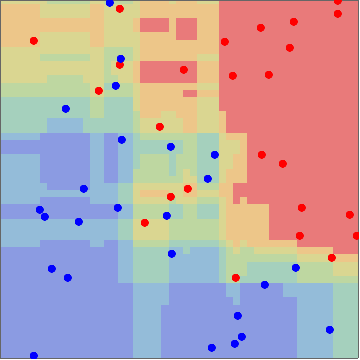
\includegraphics[width=\textwidth]{random_forest.png}
    \end{columns}
\end{frame}

\begin{frame} \frametitle{Алгоритм имитации отжига}
    \begin{center}
    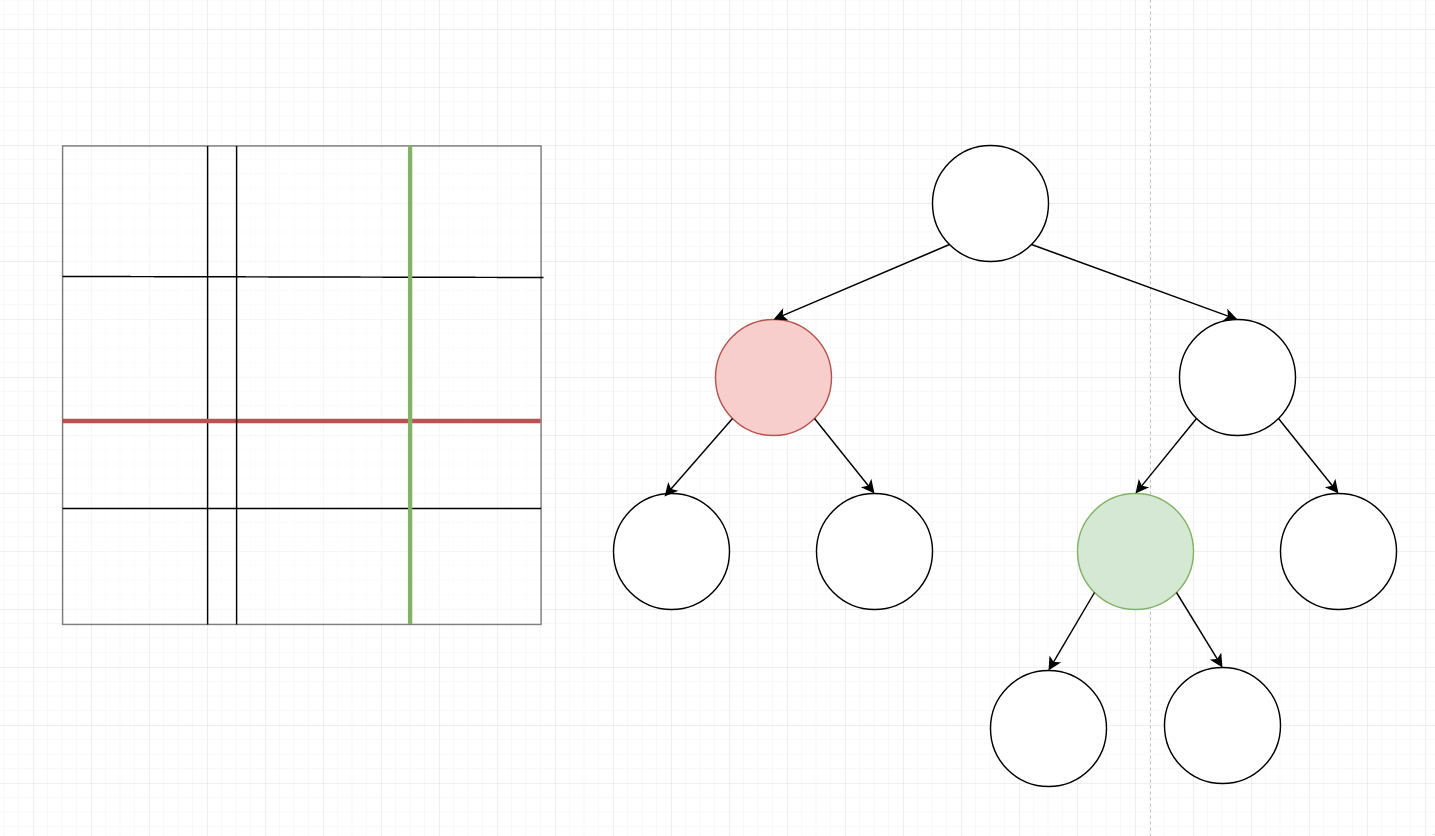
\includegraphics[width=0.8\textwidth]{gena.png}
    \end{center}
    \only<1>{%
        \begin{itemize}
            \item Разбиваем пространство по всем границам
            \item Случайные мутации по переходе в соседнюю клетку
            \item Достаточно пересчитать только одно дерево
            \item Если значение ухудшилось, то переходим с вероятностью уменьшающейся от температурного параметра
        \end{itemize}
    }
    \only<2>{%
        \begin{itemize}
            \item Рассматривает лес как 'чёрный ящик', не использует внутреннею структуру случайного леса
            \item Не работает при большом количестве признаков (>1000)
            \item Не показал желаемых результатов
        \end{itemize}
    }
\end{frame}

\begin{frame} \frametitle{Метода ветвей и границ}
    \begin{columns}
        \column{.5\textwidth}
            \begin{itemize}
                \item Перебор по всем поддеревьям
                \item Для вершины храним минимум и максимум в поддереве
                \item Поддерживаем, что все поддеревья пересекаются
            \end{itemize}
        \column{.5\textwidth}
            \begin{center}
            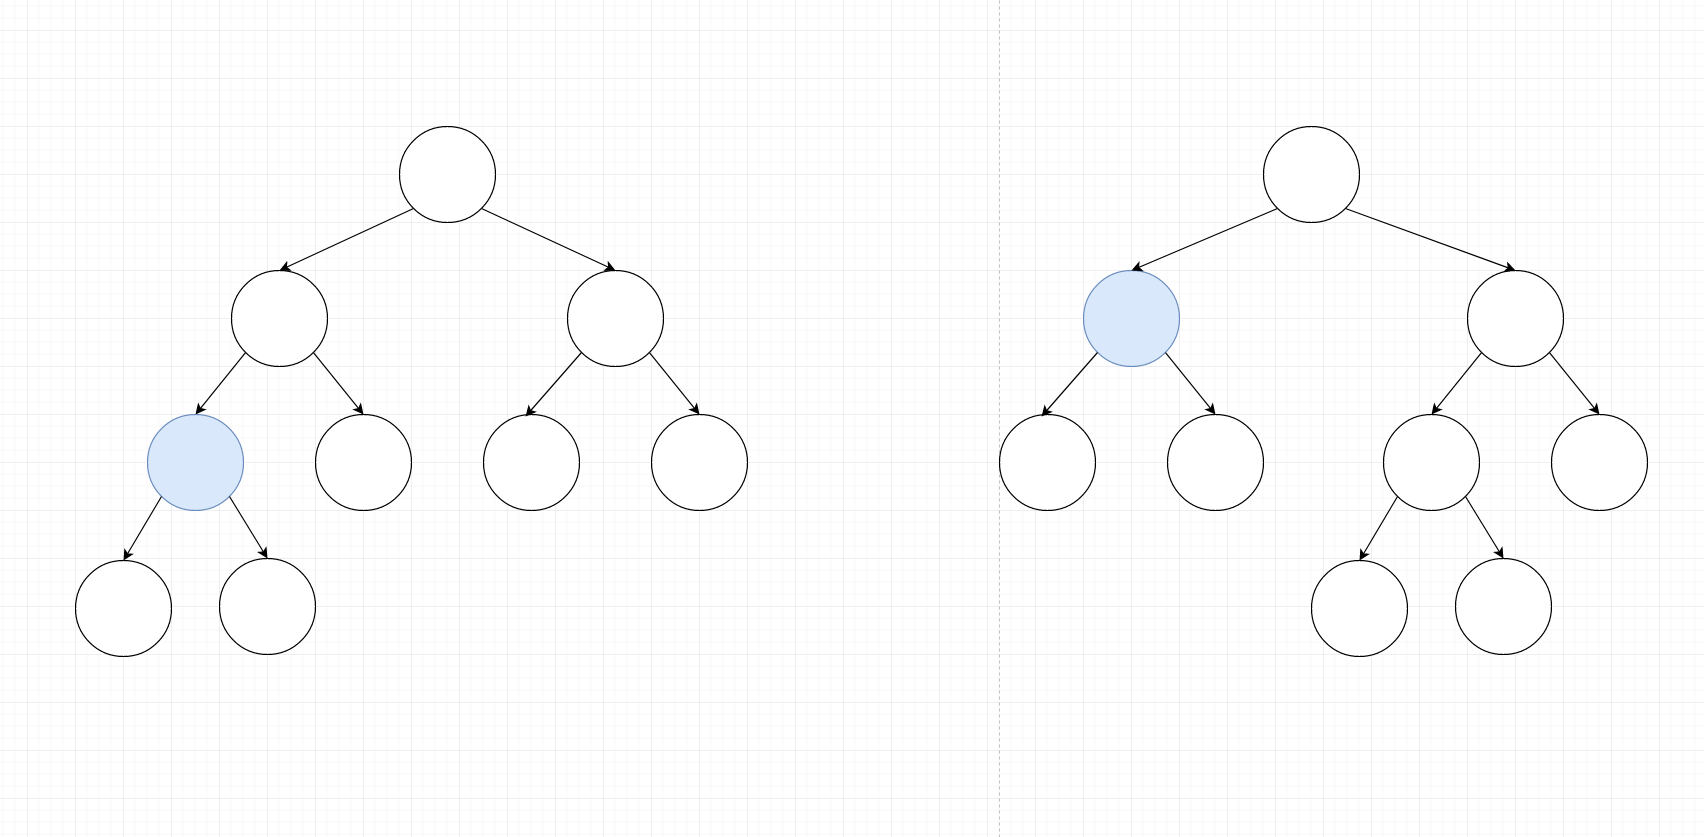
\includegraphics[height=0.8\textheight]{tree.png}

            алгоритм рассматривает синие вершины двух деревьев
            \end{center}
    \end{columns}
\end{frame}

\begin{frame} \frametitle{Метода ветвей и границ | Эвристика}

    \begin{columns}
        \column{.75\textwidth}
            На каждом шаге рассматриваем n-мерный прямоугольник области

            Шаг: разбиение по границе вершины
        \column{.25\textwidth}
            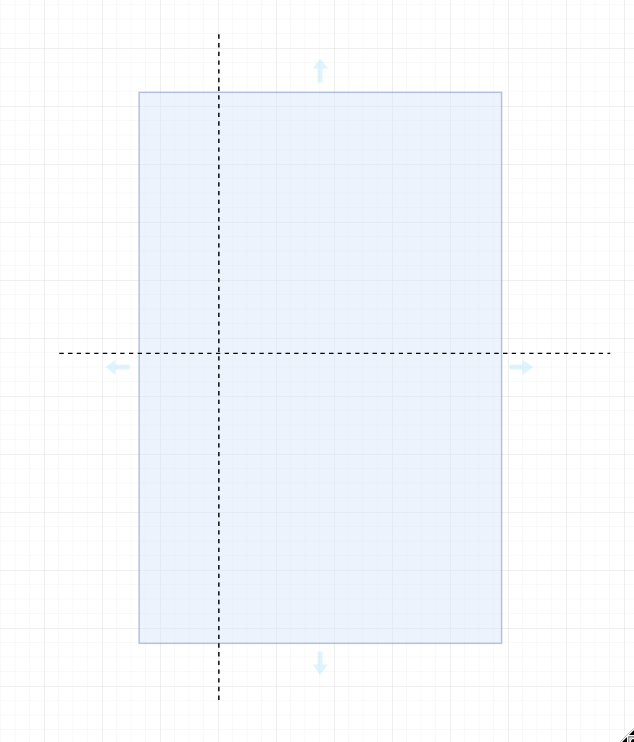
\includegraphics[width=\textwidth]{split.png}
    \end{columns}
    \vfill
    \pause{}
    Эвристика:
    \[
        i = \arg \max_{v \in trees}(|value[v.left] - value[v.right]|)
    \]
\end{frame}

\begin{frame} \frametitle{Метод ветвей и границ | Оптимизация 1}
    Необязательно искать точное решение.

    \vspace{50px}
    Не будем перебирать поддерево, если в лучшем случае это не улучшит ответ хотя бы на $\alpha$

    \[
        value[v] < \alpha current
    \]

    Гарантирует погрешность $<\alpha$
\end{frame}

\begin{frame} \frametitle{Метод ветвей и границ | Оптимизация 2}
    Максимум в поддереве может не пересекаться с текущей областью

    \begin{columns}
        \column{.5\textwidth}
            \begin{itemize}
                \item Отсортированный список всех его листьев
                \item На каждом шаге в таком списке мы движемся только вперёд
            \end{itemize}
        \column{.5\textwidth}
            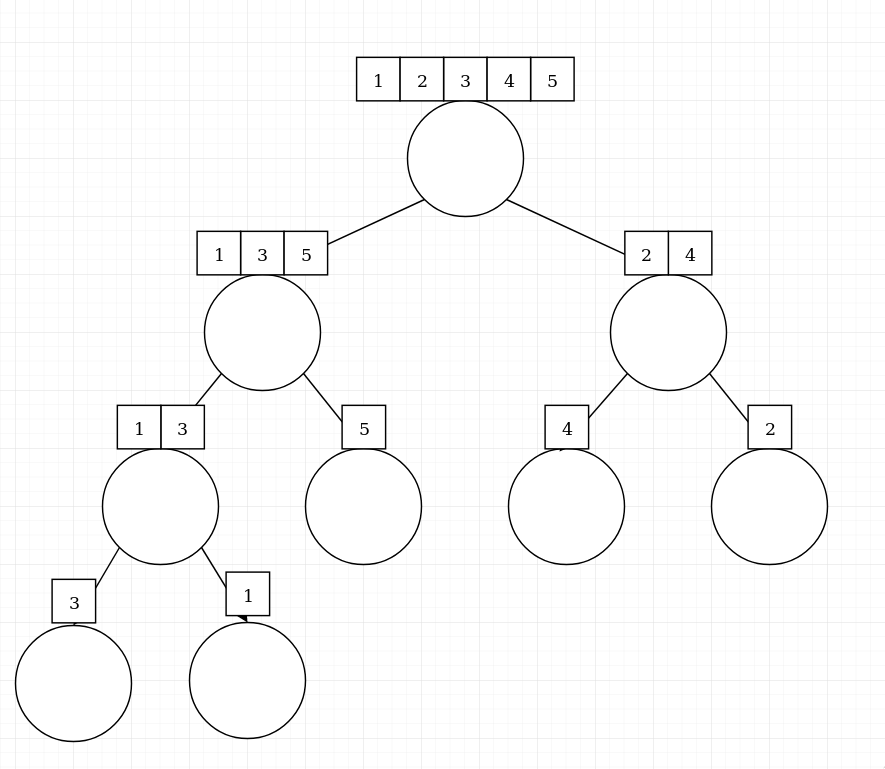
\includegraphics[width=1.1\textwidth]{merge.png}
    \end{columns}
\end{frame}

\begin{frame} \frametitle{Сравниваемые алгоритмы}
    \begin{itemize}
        \item Метод ветвей и границ 
        \item Метод ветвей и границ с погрешностью $<5\%$
        \item Случайный
        \item Отжиг
        \item Метод ветвей и границ с применением эвристики
        \item Метод ветвей и границ с применением эвристики и с погрешностью $<5\%$
        \item Метод ветвей и границ с применением эвристики и с погрешностью $<15\%$
    \end{itemize}
\end{frame}

\begin{frame} \frametitle{Использованные данные}
    Использованные различные общедоступные датасеты с OpenML

    \vfill
    \begin{center}
        \begin{tabular}{|l|l|l|}

\hline

название        & элементы  & признаки \\

\hline

diabetes        & 442    & 9     \\
boston          & 506    & 12    \\
autoPrice       & 159    & 16    \\
wisconsin       & 194    & 33    \\
strikes         & 625    & 7     \\
kin8nm          & 8192   & 9     \\
house\_8L       & 22784  & 9     \\
house\_16H      & 22784  & 9     \\
mtp2            & 274    & 1143  \\

\hline

\end{tabular}

        \vfill
        На каждом наборе параметров проводилось 10 тестов.
    \end{center}
\end{frame}

\begin{frame} \frametitle{Тестирование (Время работы | Простой случай)}
    \begin{center}
        \timeeasy{1\textwidth}{0.9\textheight}
    \end{center}
\end{frame}

\begin{frame} \frametitle{Тестирование (Время работы | Много деревьев)}
    \begin{center}
        \timetrees{1\textwidth}{0.9\textheight}
    \end{center}
\end{frame}

\begin{frame} \frametitle{Тестирование (Время работы | Большой датасет)}
    \begin{center}
        \timebig{1\textwidth}{0.9\textheight}
    \end{center}
\end{frame}

\begin{frame} \frametitle{Тестирование (Погрешность | Простой случай)}
    \begin{center}
        \erroreasy{1\textwidth}{0.9\textheight}
    \end{center}
\end{frame}

\begin{frame} \frametitle{Тестирование (Погрешность | Много признаков)}
    \begin{center}
        \errorbig{1\textwidth}{0.9\textheight}
    \end{center}
\end{frame}

\begin{frame} \frametitle{Практическое применение | Подбор гиперпараметров алгоритмов}
    \only<1>{%
        Последовательная оптимизация основанная на модели (SMBO) Sequential Model-based Algorithm configuration (SMAC)
        \begin{enumerate}
        \item Использует случайный лес в качестве регрессионной модели
        \item В лес добавляются текущие результаты алгоритмов
        \item По значениям леса выбираются новые конфигурации алгоритма
        \end{enumerate}
        Были модифицированы \texttt{automl} реализации с открытым исходным кодом: \texttt{random\_forest\_run} и \texttt{SMAC}
    }
\end{frame}

\begin{frame} \frametitle{Тестирование | SMAC}
    \begin{center}
        \smacgeneral
    \end{center}
\end{frame}

\begin{frame} \frametitle{Тестирование | SMAC, размер пространства}
    \begin{center}
        \smacsize{1\textwidth}{0.9\textheight}
    \end{center}
\end{frame}

\begin{frame} \frametitle{Тестирование | SMAC, количество запусков алгоритма}
    \begin{center}
        \smaccount{1\textwidth}{0.9\textheight}
    \end{center}
\end{frame}

\begin{frame} \frametitle{Итоги}
    \begin{itemize}
        \item Разработан алгоритм оптимизации случайного леса
        \item Проведено его сравнение с существующими методами
        \item Проверено его практическое применение в сочетании с другими алгоритмами
    \end{itemize}
\end{frame}

\end{document}
